\section{Data Link Layer}
\paragraph{Schicht 2: Sicherungsschicht}
\vspace{-1mm}
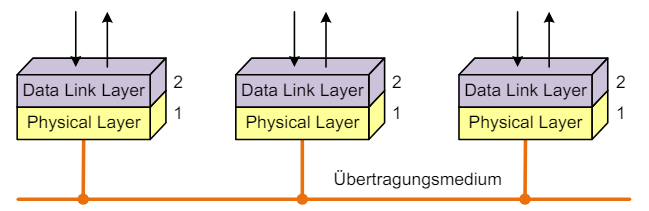
\includegraphics[width=0.5\linewidth]{images/data_link_layer.png}
\begin{definition}{Aufgaben}
    \begin{itemize}
        \item Realisieren einer zuverlässigen Verbindung zwischen Systemen
        \item Framing und Flow Control
        \item bei >2 Teilnehmern: Adressierung, Media Access, Timing
    \end{itemize}
\end{definition}

\begin{definition}{Framing (Rahmenbildung-/erkennung)}
    \begin{itemize}
        \item Senderichtung: Einpacken der zu sendenen Nutzdaten in Datenrahmen (Frames)
        \item Empfangsrichtung: Erkennung und Auspacken der Datenblöcke aus empfangenen Frames
    \end{itemize}
\end{definition}

\begin{concept}{Asynchron}\\
    Keine Daten $\rightarrow$ Nichts wird gesendet (Pause zwischen Frames)
    \begin{itemize}
        \item Zu Beginn eines Frames wird ein Start-Bit gesendet
        \item Prüfbits am Ende eines Frames!
        \item Frame-Grenze gibt auch Byte-Grenze
    \end{itemize}
    \includegraphics[width=0.8\linewidth]{images/asynchrone_übertragung_dll.png}
\end{concept}

\begin{concept}{Synchron}\\
    Frames werden ohne Unterbruch gesendet \\
    $\rightarrow$ kontinuierlicher Bitstrom auf Physical Layer
    \begin{itemize}
        \item Stehen keine Daten an, werden Flags gesendet
    \end{itemize}
    \includegraphics[width=1\linewidth]{images/synchron_übertragung_dll.png}\\
    Frames werden durch ein Start-Flag und ein End-Flag begrenzt:\\
    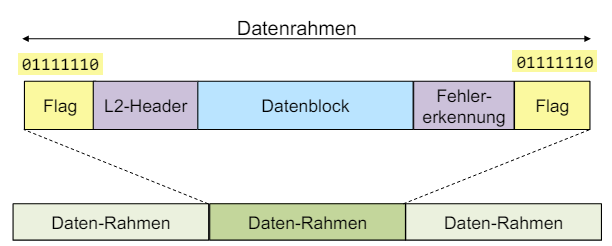
\includegraphics[width=0.7\linewidth]{images/flags_frames.png}\\
    Maskierung von Sonderzeichen (Flags) nötig!
\end{concept}

\begin{concept}{Bitstopfen}\\
    Wird verwendet um ein Bit-Muster zu garantieren.
    \begin{itemize}
        \item Sender fügt im Datenstrom nach 5 Einsen immer eine Null ein
        \item Empfänger wirft nach 5 Einsen immer ein Bit weg
        \item Somit gibt es (ausser bei Flags) die Bitfolge 01111110
    \end{itemize}
        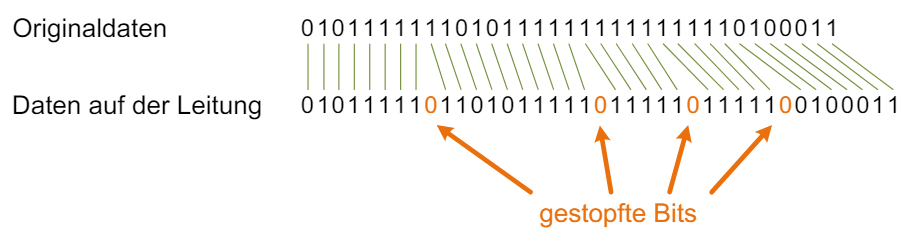
\includegraphics[width=0.8\linewidth]{images/bit_stuffing.png}
\end{concept}

\subsection{Framelänge und Fehlerwahrscheinlichkeit}

\begin{definition}{Fehlerwahrscheinlichkeit}
    BER (Bit Error Ratio):
    \begin{itemize}
        \item BER = 0.5 $\rightarrow$ jedes 2. Bit falsch
    \end{itemize}
    Weitere Definitionen:
    \begin{itemize}
        \item FER (Frame Error Ratio): Fehlerhaft empfangene Frames
        \item RER (Residual Error Ratio): Unentdeckte fehlerhafte Frames
    \end{itemize}
\end{definition}

\begin{KR}{Frame-Fehlerwahrscheinlichkeit}\\
    Wahrscheinlichkeit dass Frame der Länge N min. 1 Bitfehler enthält:\\
    BER = $p_e << 1 \longrightarrow (1 - p_e)^N \approx (1 - N \cdot p_e)$
    $$ \Rightarrow P_{Fehler, Frame} \approx N \cdot p_e (=FER)$$
\end{KR}

\begin{theorem}{Wahl der Framelänge} Kompromiss zwischen Overhead und geringer Fehlerwahrscheinlichkeit
    \begin{itemize}
    \item Lange Frames:
    \begin{itemize}
        \item Höhere Nutzdatenrate ($\uparrow$ Netto-Bitrate, $\downarrow$ Overhead)
        \item $\Uparrow$ Fehlerwahrscheinlichkeit und Datenverlust pro Fehler 
        \item $\Uparrow$ Wahrscheinlichkeit eines unentdeckten Fehlers
    \end{itemize}
    \item Kurze Frames: Tiefere Nutzdatenrate, Zuverlässig
    \end{itemize}
\end{theorem}



\begin{formula}{Framelänge}
    Nettobitrate = Bruttobitrate $\cdot \frac{Nutzdaten}{Nutzdaten + Header}$
\end{formula}

\begin{formula}{Datenraten}\\
    \begin{minipage}{0.5\linewidth}
        $$F_R = \frac{B}{8\cdot(F_L + IFG)}$$
    \end{minipage}
    \begin{minipage}{0.5\linewidth}
        $$N = F_R \cdot P \cdot 8$$
    \end{minipage}    
\end{formula}

\begin{remark}
    $F_R$ = Framerate, B = Bitrate, $F_L$ = Framelength, \\ IFG = Interframe Gap, N = Nutzbitrate, P = Payload
\end{remark}

\subsubsection{Fehlererkennung und -korrektur}

\begin{concept}{Fehlererkennung}\\
    Prinzip: Daten Redundanz hinzufügen $\rightarrow$ erhöht Hammingdistanz\\
    Zuverlässigkeit: abhängig von Framelänge und Verfahren\\
    Standards IEEE 802 (LAN-Standards, zb Ethernet):
    \begin{itemize}
        \item max. $5 \cdot 10^{-14}$ unentdeckte Fehler pro Frame-Byte
        \item BER $p_e \leq 10^{-8}$
        \item CRC32 für Ethernet, mit Generatorpolynom
    \end{itemize}
\end{concept}

\begin{concept}{Fehlerkorrektur - Error Correction (EC)}
    \begin{itemize}
        \item Backward (BEC): erneutes Übertragen der Daten
        \item Forward (FEC): Rekonstruktion von verfälschten Bits beim Empfänger
    \end{itemize}
\end{concept}

\begin{formula}{Hamming-Distanz} (h)
    \begin{itemize}
        \item Fehlererkennung: (h - 1) Fehler erkennbar
        \item Fehlerkorrektur: max. $\frac{h - 1}{2}$ Fehler korrigierbar
    \end{itemize}
\end{formula}

\begin{formula}{Einfache Parity}\\
    Prüfbit sichert ein Datenwort (typisch 1 Byte)\\
        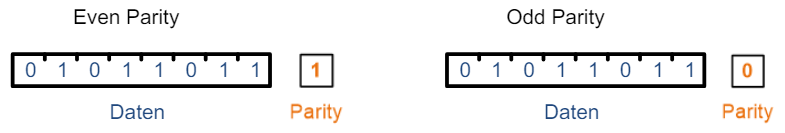
\includegraphics[width=0.9\linewidth]{images/einfache_parity.png}\\
    Even Parity: \# 1er inkl. Parity-Bit ist gerade (Odd analog)
\end{formula}

\begin{formula}{Längs- und Quer-Parity}\\
    \begin{minipage}{0.7\linewidth}
        \includegraphics[width=0.9\linewidth]{images/längs-quer-parity.png}
    \end{minipage}
    \begin{minipage}{0.25\linewidth}
        Korrigieren: \\ 1 Bit-Fehler
        \vspace*{1mm}\\
        Erkennen: \\ 2 Bit-Fehler
    \end{minipage}
\end{formula}


\subsubsection{Zugriffsmechanismen (Media Access)}

\paragraph{Gesteuerter Medium Zugriff}

\begin{definition}{Master-Slave Verfahren}\\
    Verwenden mehrere Systeme das gleiche physikalische Medium, so muss der Zugriff auf das Medium koordiniert werden
    \begin{itemize}
        \item Vorteil: Keine Konflikte, Master koordiniert Zugriff
        \item Nachteil: Ausfall des Masters (Single Point of Failure)
    \end{itemize}
\end{definition}

\begin{definition}{Token Verfahren}\\
    Die Sendeberechtigung wird in einer festgelegten Reihenfolge weitergereicht: Knoten senden nur, wenn sie ein Token halten
    \begin{itemize}
        \item Vorteil:  Deterministisch (man weiss, wann man dran kommt)
        \item Nachteil: Aufwändig (Startup, Token Verlust, etc.)
    \end{itemize}
\end{definition}

\begin{definition}{Zeitsteuerung}\\
    Zeitgesteuerter Zugriff (wie Taktfahrplan im Bahnnetz)
    \begin{itemize}
        \item Vorteil: Optimierung möglich (nach Auslastung, Durchsatz, etc.)
        \item Nachteile:
        \begin{itemize}
            \item Planung und genaue Zeit in allen Knotepunkten erforderlich
            \item Konflikte mit unplanbarem Verkehr (SBB Cargo)
        \end{itemize}
        \item Anwendungen: PROFINET IRT, Time Sensitive Networks
    \end{itemize}
\end{definition}

\paragraph{Random Medium Zugriff}

\begin{definition}{Carrier Sense Multiple Access}
    \begin{itemize}
        \item Vor dem Senden geteiltes Übertragungsmedium abhören ob frei (Carrier Sense), sonst bis zu Pause warten
        \item Vorteil: Alle Stationen gleichberechtigt (kein Master) $rightarrow$ jederzeit Zugriff auf Übertragungsmedium
        \item Nachteil: Kollisionen möglich (Collision Detection)
    \end{itemize}
\end{definition}

\begin{concept}{Kollisionsbehandlung - CSMA}
    \begin{itemize}
        \item CD (Collision Detection): Kollision $rightarrow$ abbrechen, später nochmals (ALT)
        \item CR (Collision Resolution): Hardware-unterstützte Arbitrierung (aktiv/passiv)
        \begin{itemize}
            \item Kollisionen werden erkannt und kontrolliert aufgelöst
        \end{itemize}
        \item CA (Collision Avoidance): Kollisionen vermeiden
        \begin{itemize}
            \item Request to Send / Clear to Send
        \end{itemize}
    \end{itemize}
\end{concept}

\begin{concept}{Flow-Control}\\
    Explizite Start-Stopp Signalisierung:
    \begin{itemize}
        \item Obere und untere Limite, stopp wenn oben, start wenn unten
    \end{itemize}
    Implizites Stop-and-Wait:
    \begin{itemize}
        \item Sender wartet auf Bestätigung (ACK) bevor er weiter sendet
    \end{itemize}
\end{concept}